%!TEX root = ../main.tex
\documentclass[../main.tex]{subfiles}
\begin{document}
  \chapter{Method}\label{chapter:method}

  In this chapter we review the current methods for numerically solving partial-integro differential equations. We begin by considering the simplest model for the McKendrick-von Foerster equation with constant coefficients, and a simple first order approximation to solve it.

  To further this, we consider the work of \cite{hartvig2011} who discusses a stable first order method for the McKendrick-von Foerster Equation when integral coefficients are used, but works equally well for constant coefficients. Finally we discuss the boundary conditions for the problem and adding the diffusion term to the problem.

  \section{First Order Upwind / Downwind Scheme}
  We first consider the McKendrick-von Foerster Equation with constant coefficients

  \begin{equation}
    L(u) = \frac{\partial u}{\partial t} + g \frac{\partial u}{\partial x} + \mu \cdot u
  \end{equation}

  on the discretised domain $[0, T] \times [0, W]$. By simply replacing the time derivative with a forward difference, and the spatial derivative with a backwards difference we can get a first order approximation and yields a finite difference equation

  \begin{equation}
    D^n_j(u) = \frac{u^{n+1}_j - u^n}{h} + g \frac{u^n_{j} - u^n_{j-1}}{k} + \mu u^n_j
  \end{equation}

  as an approximation to $L(u)$.

  \subsection{Courant Condition} \label{method:sec:courant}
  At this point one might question of the choice of the downwind scheme (backwards difference) as a choice for the spatial derivative. This is is ultimately for stability of the overall scheme. As discussed in \autoref{chapter:fdes} solutions to partial differential equations have an analytic domain of dependence. We saw the domain of dependence for the advection equation in \autoref{diff:fig:domainofdep} and the McKendrick-von Foerster Equation has the same domain of dependence.

  The work of \cite{courant1928} researched the idea of a \emph{Courant Number}, which in a simple terms says that the numerical domain of dependence - the region on which the numerical solution depends for information about it's solution - must contain the analytic domain of dependence.

  Formally \cite{courant1928} stated that if the Courant Number

  \begin{equation}
    C = \frac{\upsilon \delta t}{\delta x} > C_{\mbox{\small max}},
  \end{equation}

  where $\upsilon$ is the largest magnitude of velocity that information travels in the system and $C_{\mbox{\small max}}$ is a constant that depends on the approximations used (but is normally $1$), then the finite difference approximation is unstable.

  \subsection{Stability of the Scheme}
  If we are to to solve the problem $L(u) = 0$ then we can rearrange $D^n_j$ to solve for $u^{n+1}_j$, which gives a recursive formula for $\mathbf{u}^n$:

  \begin{equation} \label{method:eq:mvffde}
    u^{n+1}_j = \left(1 + h \cdot \mu - \frac{gh}{k} \right) u^n_j + \frac{gh}{k} u^n_{j-1}
  \end{equation}

  This gives us a matrix problem in the form $\mathbf{u}^{n+1} = A \mathbf{u}^n$ where

  \begin{equation}\label{method:eq:noboundary}
    A = \begin{pmatrix}
      1 + h \cdot \mu - \lambda & 0 & \\
      \lambda & 1 + h \cdot \mu - \lambda & 0 \\
        & \lambda & \ddots & \ddots & \\
        &   & \ddots & 1 + h \cdot \mu - \lambda & 0 \\
        &   &        & \lambda & 1 + h \cdot \mu - \lambda
    \end{pmatrix}
  \end{equation}

  which, using the eigenvalue method gives us a stability condition of

  \begin{equation}
    k \leq \frac{g}{\mu}.
  \end{equation}

  \subsection{Solution}
  To numerically solve the problems described in this chapter we will create a iPython notebook for each problem and produce a contour plot for each solution.

  \begin{figure}[htb]
    \centering
    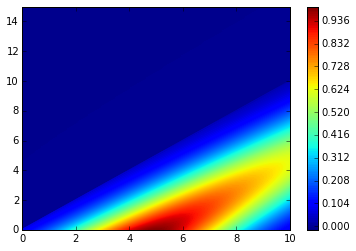
\includegraphics[width=0.5\textwidth]{_assets/advection_noPeriod.png}
    \caption{\label{method:fig:advectionPlotNoPeriod} A simulation of the advection equation with no left boundary conditions specified.}
  \end{figure}

  Using \autoref{method:eq:mvffde} as a model for iterating through each time step and a gauassian distribution as the initial condition we produce \autoref{method:fig:advectionPlotNoPeriod}, which clearly shows a decreasing solution through time. However we note that above the line $w = gt$ the solution is zero, since there has been no specified left boundary condition. This is becasue the matrix $A$ in \autoref{method:eq:noboundary} does not appropriately deal with the derivatives in the boundary. On the left boundary for $x = 0$ we find that

  \begin{equation}
    u^{n+1}_0 = \left( 1 + h \cdot \mu - \lambda \right) u^n_0,
  \end{equation}

  which is clearly not an accurate approximation for $L(u)$. While a plotting the numerical solution for this would, without further inspection shows that the left boundary is decreasing exponentially, which can be seen in \autoref{method:fig:boundayDepreciation}.

  \begin{figure}[htb]
    \centering
    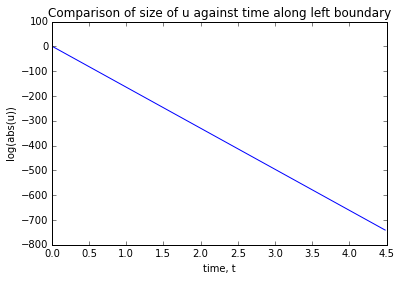
\includegraphics[width=0.5\textwidth]{_assets/uBoundary.png}
    \caption{\label{method:fig:boundayDepreciation} Size absolute value of the solution along the of left boundary.}
  \end{figure}

  To solve this issue, and throughout the problems here after, we imposed periodic boundary conditions on the domain so that

  \begin{equation}
    u(t, X_{\mathrm{Low}}) = u(t, X_{\mathrm{Hight}})
  \end{equation}

  for our choice of spatial domain $[X_{\mathrm{Low}}, X_{\mathrm{High}}]$. Biologically we can interpret this in terms of birth and death, as on the boundary $x = 0$ we have that the the approximation looks to the oldest individuals and the growth rate $g$ to determine the number of individuals who are born and have a weight less than the lower boundary on the domain. By taking $X_{\mathrm{low}} = k$ then we have that $u^n_{-1} = 0$ which is a suitable birth weight. When we add this condition the matrix $A$ is rewritten to include the extra term in the top right and

  \begin{equation}
    A = \begin{pmatrix}
      1 + h \cdot \mu - \lambda   & 0                         &         &                           & \lambda \\
      \lambda                     & 1 + h \cdot \mu - \lambda & 0       &\\
                                  & \lambda                   & \ddots  & \ddots                    & \\
                                  &                           & \ddots  & 1 + h \cdot \mu - \lambda & 0 \\
                                  &                           &         & \lambda                   & 1 + h \cdot \mu - \lambda
    \end{pmatrix}.
  \end{equation}

  A simulation confirms that the boundary conditions work as we see the solution decaying further over time and continuing the move to the right through the spatial domain for weight.

  \begin{figure}[htb]
    \centering
    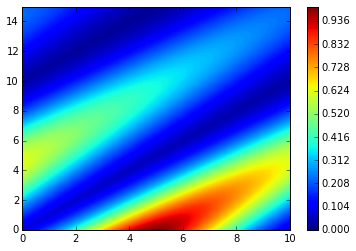
\includegraphics[width=0.5\textwidth]{_assets/advection_period.png}
    \caption{\label{method:fig:advectionPeriodic} The numerical solution of the McKendrick-von Foerster Equation with periodic boundary conditions.}
  \end{figure}

  \section{Diffusion Term \& Implicit Methods}
  Issues begin to arise when we consider the diffusion term within the upwind/downwind approximations, however \autoref{method:fig:diffusionKChange} illustrates what happens when we decrease $k < 1$ (by increasing the number of grid points with in the mesh-grid).

  \begin{figure}[htb]
    \centering
    \subfloat[Solution $k$ = 2]{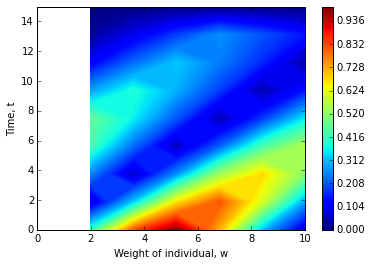
\includegraphics[width=0.45\textwidth]{_assets/diffusionLowK.png}}
    \subfloat[Solution $k$ = 0.4]{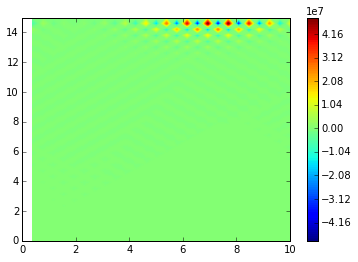
\includegraphics[width=0.45\textwidth]{_assets/diffusionHighK.png}}
    \caption{\label{method:fig:diffusionKChange} Comparison of the upwind/downwind scheme.}
  \end{figure}

  Even though the diffusion term should increase the analytic stability of the solution, we find that it also increase the instability of the numerical approximations. To solve this we take a new approach, by using implicit approximations instead of the explicit approximations.

  Instead of finding an equation for $u^{n+1}_j$ in terms of $u^n_i, i = ..., j-1, j, j+1, ... $ we aim to find an equation in the form $C \cdot \textbf{u}^{n+1} = c \cdot \textbf{u}^n$. If we begin to consider the McKendrick-von Foerster Equation with non-constant coefficients so that

  \begin{equation}
    L(u) = u_t + (g(w) \cdot u)_w + \mu(w) \cdot u
  \end{equation}

  then using the approximation from \cite{hartvig2011}, which relies upon the semi-implicit derivative for products in \cite{press1992}, we can construct a first order implicit approximation

  \begin{equation}
    D^n_j(u) = \frac{u^n_j - u^{n-1}_j}{h} + \frac{g^{n-1}_j u^n_j - g^{n-1}_{j-1} u^n_{j-1}}{k} + \mu^{n-1}_j u^n_j.
  \end{equation}

  This method is stable under the assumption that $g, \mu$ are non-linear, however we note that the approximation for the derivative in weight is only first order. To look for a higher order method we consider the average of the forwards and backwards derivatives, and add in the diffusion term to yield a finite difference equation

  \begin{equation}\label{method:eq:fullimplicit}
    D^n_j(u) = \frac{u^n_j - u^{n-1}_j}{h} + \frac{g^{n-1}_{j+1} u^n_{j+1} - g^{n-1}_{j-1} u^n_{j-1}}{2k} + \mu^{n-1}_j u^n_j - \frac{D^{n-1}_{j+1} u^n_{j+1} - 2 D^{n-1}_j u^n_j + D^{n-1}_{j-1} u^n_{j-1}}{k^2}.
  \end{equation}

  A simulation of this scheme shows the solution, while it diffuses to a stationary distribution of $u_{\mathrm{stab}}(t, x) = 0$, is calculated without numerical error and thus the scheme is stable. However we note that the inclusion of the $\mu \cdot u$ term will kill the population over time, much like the solution of the McKendrick-von Foerster Equation without diffusion. Comparing this to the solution of the equation with $\mu = 0$ we see that the solution tends to a constant over time. Closer to the solution that we aim to see earlier in \autoref{chapter:modelequations}.

  \begin{figure}[htb]
    \centering
    \subfloat[$\mu = 0.05$]{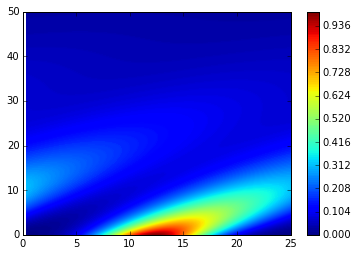
\includegraphics[width=0.5\textwidth]{_assets/diffusionSol.png}}
    \subfloat[$\mu = 0$]{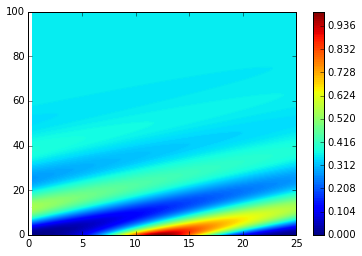
\includegraphics[width=0.5\textwidth]{_assets/diffusionSolNoDeath.png}}
    \caption{\label{method:fig:diffusionSolution} The numerical solution of the McKendrick-von Foerster Equation with periodic boundary conditions and diffusion.}
  \end{figure}

  \subsection{Integral Coefficients}
  Finally, we consider modelling the integral coefficients using the approximation in \autoref{method:eq:fullimplicit} derived from the work of \cite{hartvig2011}. However, we find that this scheme converges to the $u(t, x) = 0$ solution extremely quickly for any values of $K, \beta, \sigma, \alpha$. Evidence of this is seen in \autoref{method:fig:integralCoefficientsFail} where the solution is clearly decreasing in magnitude over time.

  \begin{figure}[htb]
    \centering
    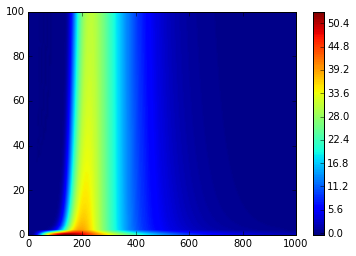
\includegraphics[width=0.5\textwidth]{_assets/integralCoeffsFail.png}
    \caption{\label{method:fig:integralCoefficientsFail} The numerical solution of the McKendrick-von Foerster Equation with periodic boundary conditions.}
  \end{figure}

  \section{Discussion}

  While problems in partial differential equation theory do have numerical methods the study of the non-linear equations is still in it's infancy and methods are not thoroughly developed. Much of the research and time spent around constructing our attempt at solving the McKendrick-von Foerster Equation with diffusion and non-linear coefficients has come from studying the problem with constants instead of functions and experimentation with approximations which are stable for those methods.

  Clearly from our study in \autoref{method:fig:diffusionKChange} and \autoref{method:fig:diffusionSolution} we see that while the diffusion term can greatly improve the stability of the solution to the equations we will need to study the death term $\mu(w) \cdot u(t, w)$ if we are to avoid this dominating the derivative and making the finite difference equation converge to a $u(t, x) = 0$ steady state solution.


\end{document}
